\Problem
{گام ششم}
{
    به تصویر خاکستری با استفاده از دستور 
    \lr{imnoise} 
    یک نویز گاوسی با میانگین صفر و پراش 
    \lr{0.01} 
    اضافه می‌کنیم.
    
    \begin{figure}[H]
        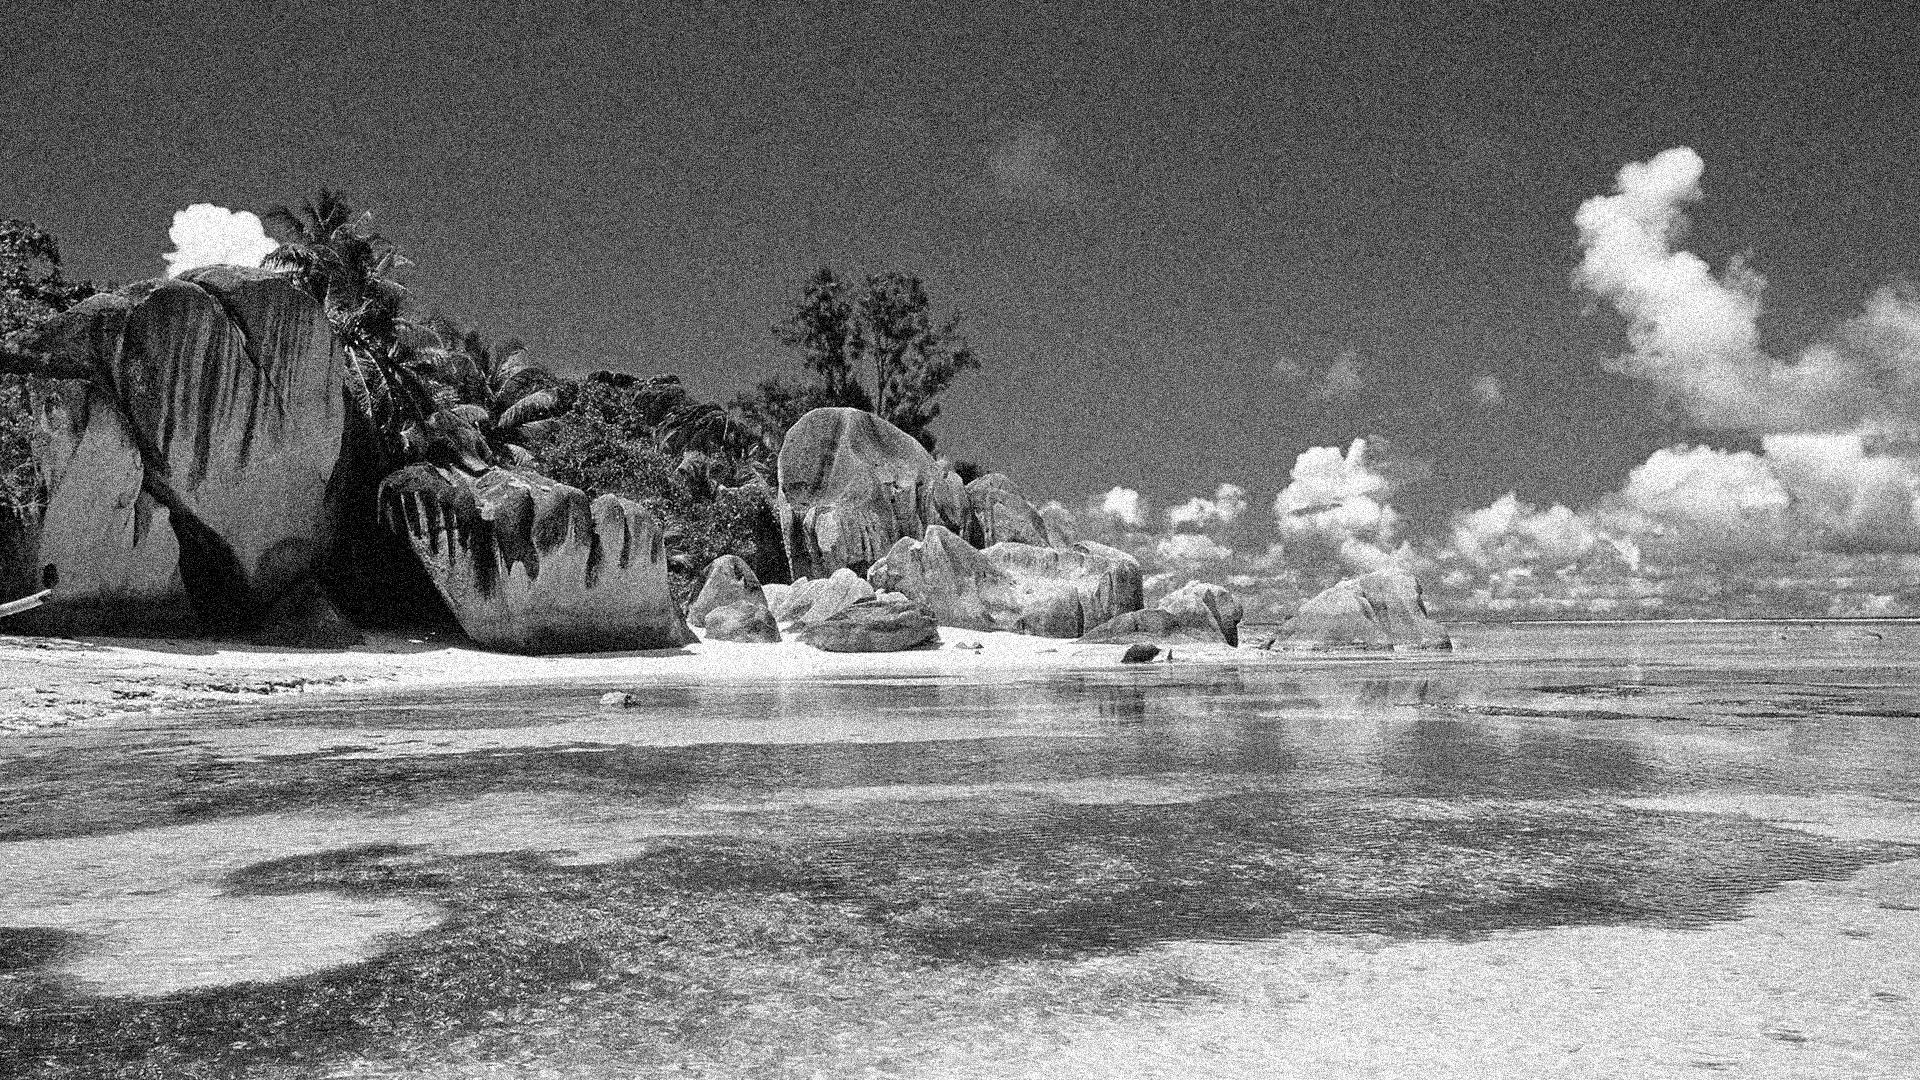
\includegraphics[width=15cm]{Images/Noisy.jpg}
        \centering
        \caption{تصویر خاکستری نویزی شده}
    \end{figure}
    
    نسبت سیگنال به نویز 
    \lr{SNR} 
    نامیده می‌شود. هرچه این مقدار بیشتر باشد یعنی نویز کمتر می‌باشد و بلعکس.
    
    برای محاسبه این نسبت دو تابع به نام‌های 
    \lr{snr.m} و \lr{snr\_elementwise.m} 
    نوشتیم که با روابط زیر این نسبت را محاسبه می‌کنند.
    
    \begin{center}
        \LTR{$SNR=\frac {\sum_{i,j} Ref(i,j)^2} {\sum_{i,j} Noise(i,j)^2}$}
        \LTR{$SNR_{ElementWise}=Average(\sum_{i,j} \frac{Ref(i,j)^2}{Noise(i,j)^2})$}
    \end{center}
    
    \RTL
    سپس مقادیر بدست آمده را به دسی‌بل تبدیل واحد می‌کنیم.
    
    \lr{Noise} 
    برابر با تفاضل سیگنال اصلی 
    \lr{Ref} 
    و سیگنال نویزی 
    \lr{Noisy} 
    می‌باشد.
    
    در حالت 
    \lr{Element Wise} 
    بعضی از المان‌های مخرج برابر صف می‌شوند و این موضوع باعث می‌شود در آن المان این نسبت به بینهایت میل پیدا کند. به‌همین دلیل از حالت اول استفاده کردیم.
    
    \newpage
    نکته: یک پیاده‌سازی دیگر برای محاسبه نسبت سیگنال به نویز وجود دارد که فقط یک ورودی می‌گیرد. نحوه کار به این صورت است که با محاسبه 3 مقدار کمینه، بیشینه و انحراف معیار در سیگنال ورودی نسبت سیگنال به نویز را محاسبه می‌کند. اما این روش مناسب سیگنال‌هایی است که توزیع نرمال گاوسی دارند. اما تصویر یک سیگنال تصادفی است و هیچ توزیع نرمالی ندارد.
    
    نکته: می‌توانستیم از تابع آماده 
    \lr{snr} 
    در متلب نیز استفاده کنیم.
    
    
    \LTR
    \lr{SNR gray image: $\infty$}
    
    \lr{PSNR gray image: $\infty$}
    
    \lr{SNR noisy image: $14.4273$ dB}
    
    \lr{PSNR noisy image: $19.9957$ dB}
    
    \RTL
    در تصویر اصلی مقادیر بینهایت بدست آمده زیرا مخرج کسر برابر صفر می‌شود.
    
}